\documentclass[12pt]{article}
\def\activityid{F05-X-v3}\usepackage[letterpaper,margin=.65in,top=.60in,bottom=.65in]{geometry}
\usepackage[T1]{fontenc}\usepackage[default]{sourcesanspro}
\usepackage{microtype,tikz,array,tabularx,fancyhdr,amsmath}\usepackage[hidelinks]{hyperref}
\usetikzlibrary{arrows.meta,calc}
\setlength{\parindent}{0pt}\setlength{\parskip}{7pt}\setlength{\headheight}{0pt}\setlength{\footskip}{26pt}\setlength{\emergencystretch}{2em}
\pagestyle{fancy}\fancyhf{}\renewcommand{\headrulewidth}{0pt}\renewcommand{\footrulewidth}{.4pt}
\fancyfoot[L]{\scriptsize Bellingham Math Circle / Week 5 / \activityid}\fancyfoot[R]{\scriptsize \thepage}
\definecolor{ink}{gray}{.12}\definecolor{soft}{gray}{.95}\color{ink}
\newcommand{\PageTitle}[2]{{\fontsize{10}{12}\selectfont\bfseries WEEK 5\quad TOWER LAB\hfill #1\par}\vspace{3pt}{\fontsize{26}{29}\selectfont\bfseries #2\par}\vspace{2pt}}
\newcommand{\Subhead}[1]{\par\vspace{3pt}{\large\bfseries #1}\par}
\newcommand{\RuleBox}[1]{\par\begingroup\setlength{\fboxsep}{8pt}\colorbox{soft}{\parbox{\dimexpr\linewidth-16pt\relax}{#1}}\endgroup\par}
\newcommand{\WriteBox}[2]{\par\textbf{#1}\par\vspace{2pt}\begin{tikzpicture}\draw[black!40,line width=.5pt] (0,0) rectangle (\dimexpr\linewidth-.5pt\relax,#2);\end{tikzpicture}\par}
\newcommand{\Code}[1]{\texttt{#1}}

\newcommand{\StudentHeader}[1]{{\fontsize{10}{12}\selectfont\bfseries Week 5 / Tower lab / #1\par}\vspace{10pt}}
\newcommand{\Problem}[2]{\par\vspace{4pt}\textbf{Problem #1:} #2\par}
\newcommand{\RecordBox}[2]{\par #1\par\vspace{2pt}\begin{tikzpicture}\draw[black!40,line width=.5pt](0,0)rectangle(\dimexpr\linewidth-.5pt\relax,#2);\end{tikzpicture}\par}

\hypersetup{pdftitle={Week 5: Extra / Grades 6--7}}
\begin{document}
\StudentHeader{Extra / Grades 6--7}
\Problem{1}{Copy this city. Every row and column must contain 1--4 once. In the upper-left bold block, exchange the 1s and 2s. Record the changed city on the right, then check each row and column.}
\begin{center}\begin{minipage}{.48\linewidth}\centering 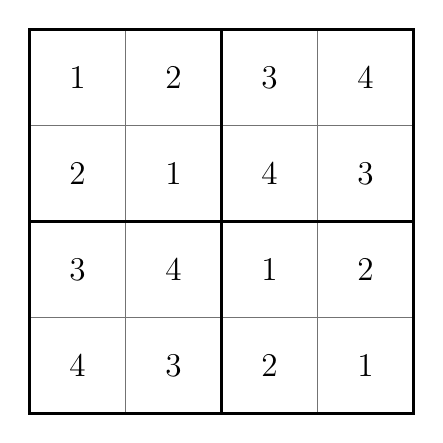
\begin{tikzpicture}[x=0.48in,y=0.48in]\draw[step=1,black!55](0,0)grid(4,4);\draw[thick](0,0)rectangle(4,4);\draw[line width=1.3pt](2,0)--(2,4)(0,2)--(4,2);\node[font=\large]at(0.5,3.5){1};\node[font=\large]at(1.5,3.5){2};\node[font=\large]at(2.5,3.5){3};\node[font=\large]at(3.5,3.5){4};\node[font=\large]at(0.5,2.5){2};\node[font=\large]at(1.5,2.5){1};\node[font=\large]at(2.5,2.5){4};\node[font=\large]at(3.5,2.5){3};\node[font=\large]at(0.5,1.5){3};\node[font=\large]at(1.5,1.5){4};\node[font=\large]at(2.5,1.5){1};\node[font=\large]at(3.5,1.5){2};\node[font=\large]at(0.5,0.5){4};\node[font=\large]at(1.5,0.5){3};\node[font=\large]at(2.5,0.5){2};\node[font=\large]at(3.5,0.5){1};\end{tikzpicture}\end{minipage}\hfill\begin{minipage}{.48\linewidth}\centering 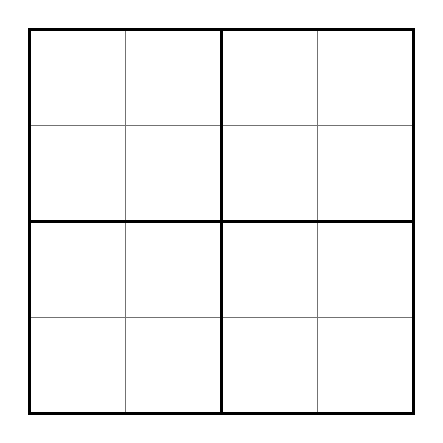
\begin{tikzpicture}[x=0.48in,y=0.48in]\draw[step=1,black!55](0,0)grid(4,4);\draw[thick](0,0)rectangle(4,4);\draw[line width=1.3pt](2,0)--(2,4)(0,2)--(4,2);\end{tikzpicture}\end{minipage}\end{center}
\Problem{2}{Start from the original city each time. Switch the two heights within just one other bold block. Record each changed city below. Check every row and column after each switch.}
\begin{center}\begin{tabular}{ccc}Upper right&Lower left&Lower right\\[5pt]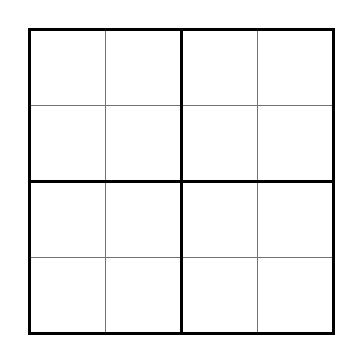
\begin{tikzpicture}[x=0.38in,y=0.38in]\draw[step=1,black!55](0,0)grid(4,4);\draw[thick](0,0)rectangle(4,4);\draw[line width=1.3pt](2,0)--(2,4)(0,2)--(4,2);\end{tikzpicture}&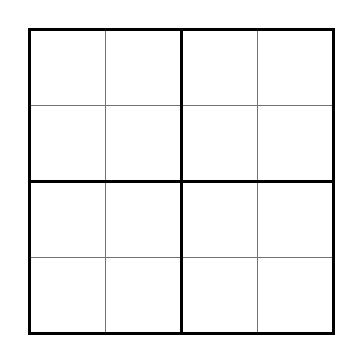
\begin{tikzpicture}[x=0.38in,y=0.38in]\draw[step=1,black!55](0,0)grid(4,4);\draw[thick](0,0)rectangle(4,4);\draw[line width=1.3pt](2,0)--(2,4)(0,2)--(4,2);\end{tikzpicture}&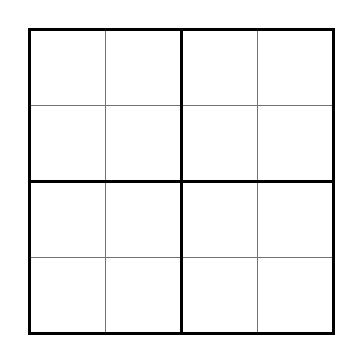
\begin{tikzpicture}[x=0.38in,y=0.38in]\draw[step=1,black!55](0,0)grid(4,4);\draw[thick](0,0)rectangle(4,4);\draw[line width=1.3pt](2,0)--(2,4)(0,2)--(4,2);\end{tikzpicture}\end{tabular}\end{center}
\RecordBox{Rows and columns affected by my lower-left switch:}{0.65in}

\newpage
\StudentHeader{Extra / Grades 6--7}
\Problem{3}{An entry clue fixes the height in one cell. There are no outside clues on this page. Copy the original city from Problem 1. Circle three cells as clues. Choose a bold block with no circled cell. Switch its two heights, then check that all three clues still hold. Repeat using a different choice of three clues.}
\begin{center}\begin{minipage}{.48\linewidth}\centering 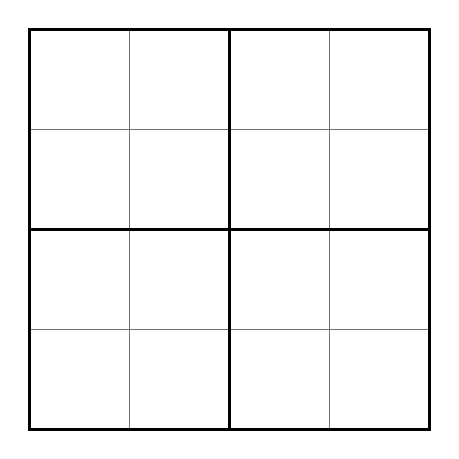
\begin{tikzpicture}[x=0.5in,y=0.5in]\draw[step=1,black!55](0,0)grid(4,4);\draw[thick](0,0)rectangle(4,4);\draw[line width=1.3pt](2,0)--(2,4)(0,2)--(4,2);\end{tikzpicture}\end{minipage}\hfill\begin{minipage}{.48\linewidth}\centering 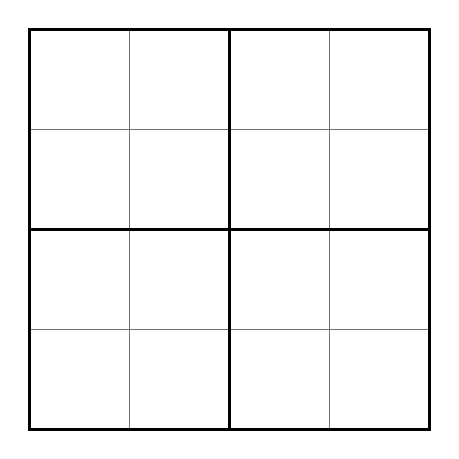
\begin{tikzpicture}[x=0.5in,y=0.5in]\draw[step=1,black!55](0,0)grid(4,4);\draw[thick](0,0)rectangle(4,4);\draw[line width=1.3pt](2,0)--(2,4)(0,2)--(4,2);\end{tikzpicture}\end{minipage}\end{center}
\Problem{4}{Now keep the four entries shown below. They touch all four bold blocks. Build two different cities that keep these entries and use 1--4 once in every row and column.}
\begin{center}\begin{minipage}{.48\linewidth}\centering 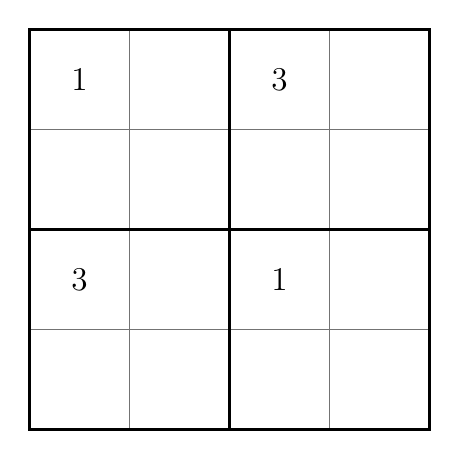
\begin{tikzpicture}[x=0.5in,y=0.5in]\draw[step=1,black!55](0,0)grid(4,4);\draw[thick](0,0)rectangle(4,4);\draw[line width=1.3pt](2,0)--(2,4)(0,2)--(4,2);\node[font=\large]at(0.5,3.5){1};\node[font=\large]at(2.5,3.5){3};\node[font=\large]at(0.5,1.5){3};\node[font=\large]at(2.5,1.5){1};\end{tikzpicture}\end{minipage}\hfill\begin{minipage}{.48\linewidth}\centering 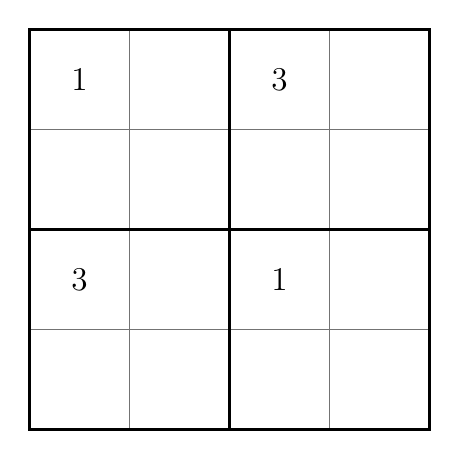
\begin{tikzpicture}[x=0.5in,y=0.5in]\draw[step=1,black!55](0,0)grid(4,4);\draw[thick](0,0)rectangle(4,4);\draw[line width=1.3pt](2,0)--(2,4)(0,2)--(4,2);\node[font=\large]at(0.5,3.5){1};\node[font=\large]at(2.5,3.5){3};\node[font=\large]at(0.5,1.5){3};\node[font=\large]at(2.5,1.5){1};\end{tikzpicture}\end{minipage}\end{center}
\RecordBox{Cells I changed while keeping the four clues:}{0.6in}

\end{document}
